\documentclass[tikz,border=2pt]{standalone}
\usepackage{amsmath}
\usetikzlibrary{arrows.meta}
\begin{document}
% Characteristic roots of the page's examples in the complex plane. Asymptotic stability needs every root
% in the open left half-plane: -1, -2 (x''+3x'+2x=4) yes; +-2i (x''+4x=0) on the axis, bounded only;
% 1 +- 2i (x''-2x'+5x=0) and the double root 0 (x''=0) unstable.
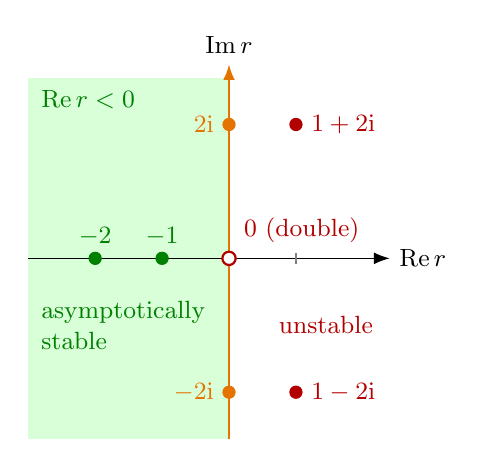
\begin{tikzpicture}[font=\small, >={Latex[length=2mm]}, x=0.85cm, y=0.85cm]
  \fill[green!15] (-3.0,-2.7) rectangle (0,2.7);
  \draw[->] (-3.0,0) -- (2.4,0) node[right] {$\operatorname{Re} r$};
  \draw[->, orange!90!black, thick] (0,-2.7) -- (0,2.9) node[above, black] {$\operatorname{Im} r$};
  \foreach \y in {-2,2} \draw[gray] (-0.08,\y) -- (0.08,\y);
  \foreach \x in {-2,-1,1} \draw[gray] (\x,-0.08) -- (\x,0.08);
  \node[green!50!black, anchor=north west] at (-2.95,2.65) {$\operatorname{Re} r<0$};
  \node[green!50!black, anchor=west, align=left] at (-2.95,-1.0) {asymptotically\\ stable};
  \node[red!70!black, anchor=west] at (0.6,-1.0) {unstable};
  % stable roots
  \fill[green!50!black] (-1,0) circle (2.4pt) node[above, yshift=1pt] {$-1$};
  \fill[green!50!black] (-2,0) circle (2.4pt) node[above, yshift=1pt] {$-2$};
  % purely imaginary pair
  \fill[orange!90!black] (0,2) circle (2.4pt) node[left, xshift=-2pt] {$2\mathrm{i}$};
  \fill[orange!90!black] (0,-2) circle (2.4pt) node[left, xshift=-2pt] {$-2\mathrm{i}$};
  % unstable roots
  \fill[red!70!black] (1,2) circle (2.4pt) node[right, xshift=2pt] {$1+2\mathrm{i}$};
  \fill[red!70!black] (1,-2) circle (2.4pt) node[right, xshift=2pt] {$1-2\mathrm{i}$};
  \draw[red!70!black, thick, fill=white] (0,0) circle (2.4pt);
  \node[red!70!black, anchor=south west] at (0.08,0.08) {$0$ (double)};
\end{tikzpicture}
\end{document}
